\documentclass[12pt,]{article}
\usepackage[left=1in,top=1in,right=1in,bottom=1in]{geometry}
\newcommand*{\authorfont}{\fontfamily{phv}\selectfont}
\usepackage[]{mathpazo}


  \usepackage[T1]{fontenc}
  \usepackage[utf8]{inputenc}




\usepackage{abstract}
\renewcommand{\abstractname}{}    % clear the title
\renewcommand{\absnamepos}{empty} % originally center

\renewenvironment{abstract}
 {{%
    \setlength{\leftmargin}{0mm}
    \setlength{\rightmargin}{\leftmargin}%
  }%
  \relax}
 {\endlist}

\makeatletter
\def\@maketitle{%
  \newpage
%  \null
%  \vskip 2em%
%  \begin{center}%
  \let \footnote \thanks
    {\fontsize{18}{20}\selectfont\raggedright  \setlength{\parindent}{0pt} \@title \par}%
}
%\fi
\makeatother




\setcounter{secnumdepth}{0}

\usepackage{longtable,booktabs}

\usepackage{graphicx,grffile}
\makeatletter
\def\maxwidth{\ifdim\Gin@nat@width>\linewidth\linewidth\else\Gin@nat@width\fi}
\def\maxheight{\ifdim\Gin@nat@height>\textheight\textheight\else\Gin@nat@height\fi}
\makeatother
% Scale images if necessary, so that they will not overflow the page
% margins by default, and it is still possible to overwrite the defaults
% using explicit options in \includegraphics[width, height, ...]{}
\setkeys{Gin}{width=\maxwidth,height=\maxheight,keepaspectratio}


\title{Political Donor Polarization in Wisconsin \thanks{Code and data available at: github.com/rossdahlke}  }



\author{\Large Ross Dahlke\vspace{0.05in} \newline\normalsize\emph{}  }


\date{}

\usepackage{titlesec}

\titleformat*{\section}{\normalsize\bfseries}
\titleformat*{\subsection}{\normalsize\itshape}
\titleformat*{\subsubsection}{\normalsize\itshape}
\titleformat*{\paragraph}{\normalsize\itshape}
\titleformat*{\subparagraph}{\normalsize\itshape}





\newtheorem{hypothesis}{Hypothesis}
\usepackage{setspace}


% set default figure placement to htbp
\makeatletter
\def\fps@figure{htbp}
\makeatother


% move the hyperref stuff down here, after header-includes, to allow for - \usepackage{hyperref}

\makeatletter
\@ifpackageloaded{hyperref}{}{%
\ifxetex
  \PassOptionsToPackage{hyphens}{url}\usepackage[setpagesize=false, % page size defined by xetex
              unicode=false, % unicode breaks when used with xetex
              xetex]{hyperref}
\else
  \PassOptionsToPackage{hyphens}{url}\usepackage[draft,unicode=true]{hyperref}
\fi
}

\@ifpackageloaded{color}{
    \PassOptionsToPackage{usenames,dvipsnames}{color}
}{%
    \usepackage[usenames,dvipsnames]{color}
}
\makeatother
\hypersetup{breaklinks=true,
            bookmarks=true,
            pdfauthor={Ross Dahlke ()},
             pdfkeywords = {state politics, political donations, network analysis, polarization},  
            pdftitle={Political Donor Polarization in Wisconsin},
            colorlinks=true,
            citecolor=blue,
            urlcolor=blue,
            linkcolor=magenta,
            pdfborder={0 0 0}}
\urlstyle{same}  % don't use monospace font for urls

% Add an option for endnotes. -----


% add tightlist ----------
\providecommand{\tightlist}{%
\setlength{\itemsep}{0pt}\setlength{\parskip}{0pt}}

% add some other packages ----------

% \usepackage{multicol}
% This should regulate where figures float
% See: https://tex.stackexchange.com/questions/2275/keeping-tables-figures-close-to-where-they-are-mentioned
\usepackage[section]{placeins}


\begin{document}
	
% \pagenumbering{arabic}% resets `page` counter to 1 
%
% \maketitle

{% \usefont{T1}{pnc}{m}{n}
\setlength{\parindent}{0pt}
\thispagestyle{plain}
{\fontsize{18}{20}\selectfont\raggedright 
\maketitle  % title \par  

}

{
   \vskip 13.5pt\relax \normalsize\fontsize{11}{12} 
\textbf{\authorfont Ross Dahlke} \hskip 15pt \emph{\small }   

}

}








\begin{abstract}

    \hbox{\vrule height .2pt width 39.14pc}

    \vskip 8.5pt % \small 

\noindent American politics has recently been defined by unprecedented levels of
partisan polarization. Given the concurrent rise of the amount of money
in politics, there is a natural connection that many people make between
money in politics and polarization. This paper uses the occurence of a
specific event, former Wisconsin Governor Scott Walker's introduction
and passage of Act 10 and subsequent protests and recall election, to
analyze the relationship between donor polarization and mass
polarization. The data show that political donor networks polarized
during the 2012 election cycle at the same time as the mass electorate.
This result suggests that politic donors were likely not the cause of
the polarization in the state and provides evidence for the
`consumption' model of political donations.


\vskip 8.5pt \noindent \emph{Keywords}: state politics, political donations, network analysis, polarization \par

    \hbox{\vrule height .2pt width 39.14pc}



\end{abstract}


\vskip -8.5pt


 % removetitleabstract

\noindent \doublespacing 

Political campaign finance plays an important role in the American
political system. This significance is evidenced by the attention that
academic researchers pay to the topic as well as the many different
contexts in which campaign finance is studied. For example, research has
been conducted on the impact of political donations on roll-call voting
in the U.S. Congress (Roscoe and Jenkins 2005; Stratmann 1991), gender
representation in political parties (Crowder-Meyer and Cooperman 2018;
Barber, Butler, and Preece 2016; Kitchens and Swers 2016; Thomsen and
Swers 2017), ability to win political campaigns (Bonica 2017; Bonneau
2007), the connection between money raised and public attention (Ellis,
Ripberger, and Swearingen 2017), judicial function (Palmer and Levendis
2008), perceptions of corruption (Bowler and Donovan 2015), political
economy and stock returns (Akey 2015; Fowler, Garro, and Spenkuch 2020;
Cooper, Gulen, and Ovtchinnikov 2010), and the significant amount of
time that candidates and legislators devote to fundraising
(Torres-Spelliscy 2017).

Even though political donors are believed to play an out-sized role in
democracy, the psychological processes of donors is thought to be
similar to voters. Political donations can be thought of an extension of
voting. In other words, both actions are political consumptions that
seek to improve their preferred candidate's chances of winning.
Ansolabehere, de Figueiredo and Snyder summarized this idea by stating,
``In our view, campaign contributing should not be viewed as an
investment, but rather as a form of consumption--or, in the language of
politics, participation'' (Ansolabehere, Figueiredo, and Jr. 2003).
Donations can be seen as an outlet for motivated citizens to increase
their participation beyond just turning out to vote when they perceive
the stakes of elections to be high (Hill and Huber 2017).

The folk-theory of political donors is of smokey backrooms and
access-oriented donors who seek to have a direct influence on policy
making. However, even when donors contribute to legislators that
maximize their economic interests, donations are not found to be
motivated by existing policy agreements and not an expectation of access
(Barber, Canes-Wrone, and Thrower 2016). Even donations from business
executives have been found to be ``best understood as purchases of `good
will' whose returns, while positive in expectation, are contingent and
rare'' (Gordon, Hafer, and Landa 2007).

Although the psychological process of making a political campaign
contribution can be thought of as similar to voting, there are
significant demographic and ideological differences between donors and
voters. People with lower incomes, less education, and do not work in
professional and managerial jobs are less likely to be politically
engaged, including making political donations (Laurison 2016). Donors to
the Democratic and Republican parties were summarized as being
``Limousine Liberals'' and ``Corporate Conservatives'' (Francia et al.
2005).In addition, Democrats and Republicans draw their bases of
electoral support from different geographic bases. However, major
campaign donors are highly concentrated geographically. These
``big-donor neighborhoods'' are unrepresentative of the country as a
whole and point to these communities having a distinct political culture
(Bramlett, Gimpel, and Lee 2011). In both parties, donors are more
ideologically extreme than non-donating voters, even among primary
voters (Hill and Huber 2017; Francia et al. 2003). Even wealthy donors
who make up the ``big money'' in politics are very partisan (McCarty,
Poole, and Rosenthal 2006).

This ideological extremity shown by political donors has led some
scholars to suggest that political donors are contributors to the
partisan polarization of the politics of the United States (Francia et
al. 2005). This speculation that that political donors are contributors
of polarization is bolstered by the observation that both political
polarization and campaign spending have risen in conjunction (McCarty,
Poole, and Rosenthal 2006). However, there little evidence for the
causal relationship of donors causing political polarization. And many
have concluded that political donations don't influence polarization
(Harden and Kirkland 2016; Raja and Wiltse 2012; Keena and Knight-Finley
2019). Furthermore, it is likely the case that the causal arrow flows
the other direction, and it is more polarized candidates and electorate
that have led to more polarized donors (Harden and Kirkland 2016; Raja
and Wiltse 2012; Keena and Knight-Finley 2019).

Studying polarization, particularly among political donors can be
difficult because of the myriad of potential confounding factors that
can contribute to polarization (Harden and Kirkland 2016). In addition,
polarization is generally a phenomenon that gradually increases or
decreases over time (Center 2017). However, this paper leverages a
singular event, former Wisconsin Governor Scott Walker's proposition and
passage of Act 10, a ``budget repair bill'' that ended collective
bargaining for teachers unions and the subsequent protests and recall
election, to examine political donor polarization in the state of
Wisconsin. Given the recent research which has pointed to the
polarization of political donors as being \emph{reactive} instead of
\emph{causal} to broader polarization, we could expect political donors
to follow the trend of voters and polarize after introduction of Act 10
and subsequent events.

\textbf{H1: Political donors in the State of Wisconsin polarized during
the 2011-2012 election cycle compared to the 2009-2010 election cycle
and maintained their level of polarization in the 2013-2014 election
cycle.}

If hypothesis one is found to be correct, these results would strengthen
the evidence for politics donors being \emph{reactive} to their
political environment as we would expect under Ansolabehere, de
Figueiredo and Snyder's consumption model of political giving.

Alternatively, if political donors are contributors to polarization, as
is suggested by some scholars, we would expect to see hypothesis 2.

\textbf{H2: Polarization levels stays the same from 2009-2010 compared
to 2011-2012.}

If hypothesis two is upheld, the result would suggest that political
donors helped to create the polarized political environment that we see
today.

In addition, this paper makes a methodological contribution to the field
of political polarization studies by taking a network approach to
measuring polarization to similar to studies of congressional
polarization (Waugh et al., n.d., @zhang2008) and polarization in social
media networks (Guerra et al. 2013; Garcia et al. 2015; Conover et al.
2011) and uses modularity as a measure of polarization within political
donor networks. This paper conceives of the political donor landscape of
donors and candidates acting as nodes who are connected by donations
made that act as edges. This method is important in studying political
donor networks because it takes into consideration real-world actions,
such as in the study of polarization among member of congress where
voting records (Guerra et al. 2013) and co-sponsorships (Zhang et al.
2008), which are used to study polarization opposed to surveys
administered to donors that rely on self-reported ideology and
partisanship.

\hypertarget{wisconsin-context}{%
\section{Wisconsin Context}\label{wisconsin-context}}

Both Wisconsin's legislators and mass public are among the most
polarized in the nation (Cramer 2016) and has been used by academics as
an example of how political actions change in contenious and divisive
environments (Bode et al. 2018). Although many state legislatures are
also experiencing polarization (Shor 2015), Wisconsin is unique in that
there is a single event that many point to in creating ``the most
politically divisive place in America'' (Kaufman 2012).

In 2011, newly-elected Republican Governor Scott Walker introduced Act
10, a ``budget reconciliation bill'' that among other cuts to funding,
stripped public school teachers of collective bargaining via their
union. Up to 100,000 protested this ``anti-union bill'' at the State
Capitol and even occupied the capitol building for a period of time
(Sewell 2011). Democratic lawmakers fled to Illinois in an effort to
delay or stop the bill from passing into law (Layton 2011). In 2012
there was an unsuccessful election to recall Governor Walker.

Wisconsin Governor Scott Walker's self-anointed ``divide and conquer''
politics (Blake 2012) has left a political divide in Wisconsin that
persists to today. The result is that ``divisive politics ruled
Wisconsin over the last decade'' (Marley and Beck 2019). The Marquette
Law School poll headed by Charles Franklin has called public opinion in
Wisconsin a ``lesson in the two worlds of Wisconsin'' where ``it seems
often as if people have not only differing opinions but differing views
of facts and realities'' (Borsuk 2017).

\hypertarget{methodology}{%
\section{Methodology}\label{methodology}}

All data on political contributions came from the Wisconsin Campaign
Finance Information System (CFIS). I exported all contributions to State
Assembly, State Senate, and Gubernatorial races from the 2010, 2012, and
2014 elections. This dataset does not include donations to party
committees, although it does include disbursements from these
committees. I manually created a table of the parties of each of all the
campaigns receiving contributions in this timeframe and added the party
of the campaign receiving the donation to this dataset.

I started with 1,499,603 donations. To clean the data, I filtered out
3,503 unitemized/ anonymous donations , removed punctuation from the
names of the donors, and used Open Refine via the \texttt{refiner} R
package to standardize names (for example, Jim versus James). Next, I
created a unique identifier for donors by combining their standardized
name with their zip code. This identifier was created to be able to link
donors who contributed across multiple campaigns in multiple years
without considering two different people, with the same name, from
different locations to be the same person.

Next, I derived the partisanship of each donor in each election cycle. I
calculated each donor's partisanship by taking the percent of donations
that each donor gave to Republicans divided by their donations to
Republicans and Democrats. I took that ``percent donated to
Republicans'' and rescaled it from -1 to 1, where -1 represents the most
Democratic donors, and 1 the most Republican donors. I also calculated
each individual's party bin: if more than 75\% of donations were to
Democrats, they were labeled as a Democrat; if more than 75\% of
donations were to Republicans, they were labeled as a Republican; if
their donations were somewhere inbetween, they were labeled as being a
bipartisan donor.

To quantify the levels of polarization in each election cycle, I
calculated two statistics: network modularity and average absolute
partisanship of donors.

First, political donations can be thought of as a network where donors
and candidates are nodes and donations connecting donors and candidates
are edges. This conceptualization of the political donor landscape as
network allows us to examine the network structure and calculate network
statistics on the graph of donors and candidates. One of the most useful
network statistics for measuring polarization in a network's modularity.

The modularity of a graph measures how good the division of groups (such
as political parties) is by calculating ``the number of edges falling
within groups minus the expected number in an equivalent network with
edges placed at random'' (Newman 2006). The modularity of a network
falls in range {[}-1/2, 1{]}. If the modularity is positive, the number
of edges that remain within each group is greater than the expected
number to remain in-group based on chance. The higher the modularity,
the greater the concentration of edges within each groups. In other
words, the higher the modularity of a network, the higher the
polarization among the groups. Formally, the equation to calculation
modularity Q is:

\[Q = \frac{1}{2m} \sum_{ij}\left[A_{ij} - \frac{k_{i}k_{j}}{2m} \right]\delta(g_{i},g_{j})\]

In this equation \(m = \frac{1}{2}\sum_{i}k_{i}\) is equal to the
``total strength of ties in the network'', \(k_{i}=\sum_{j}A_{ij}\) is
the strength/ weighted degree of the \(i\)th node, \(g_{i}\) is the
group (in this case, party/ party bin) to which the \(i\) belong, and
\(\delta(g_{i},g_{j}) = 1\) if \(i\) and \(j\) belong to the same group
(party/ party bin) and 0 if they do not belong to the same party/ party
bin (Waugh et al., n.d.).

I calculated the modularity of the network graphs of each election cycle
(2010, 2012, 2014) using the \texttt{igraph} R package (Csardi and
Nepusz 2006). I used candidates' declared parties and donors' party bin
as the groups for the modularity calculation. The modularity of the
network graph of each election is in Table 1.

In addition to calculating the change in modularity of each of the
election cycles, I also analyzed the change in mean absolute
partisanship of the donors in each election cycle.

I defined a donor's absolute partisanship as the absolute value of their
partisanship score (which is on a scale from -1 to 1). Therefore, the
larger a donor's absolute the partisanship, the higher percentage of
their money that they contributed to a single party. To calculate the
significance in the difference of the mean absolute partisanship, I use
a bootstrap methodology with 1000 replications. This paper uses a
non-parametric bootstrap/ resampling method because of the non-normal
distribution of partisanship of the donors given that a strong majority
(98\%) of donors in a given election cycle only contribute to a single
party. The results of the bootstrap are found in Table 2.

\newpage

\hypertarget{tables}{%
\section{Tables}\label{tables}}

\hypertarget{table-1}{%
\subsubsection{Table 1}\label{table-1}}

\begin{longtable}[]{@{}lr@{}}
\caption{Tbl. 1: Modularity calculation for the donor networks in each
election cycle. Higher modularity means more
polarization}\tabularnewline
\toprule
Election Cycle & Modularity\tabularnewline
\midrule
\endfirsthead
\toprule
Election Cycle & Modularity\tabularnewline
\midrule
\endhead
2010 & 0.3987161\tabularnewline
2012 & 0.4912335\tabularnewline
2014 & 0.4797870\tabularnewline
\bottomrule
\end{longtable}

\newpage

\hypertarget{table-2}{%
\subsubsection{Table 2}\label{table-2}}

\begin{longtable}[]{@{}lrll@{}}
\caption{Tbl. 2: Bootstrapped difference-in-means test with 1,000
replications comparing mean partisanship of donors.}\tabularnewline
\toprule
Election Cycle & T & CI & p\tabularnewline
\midrule
\endfirsthead
\toprule
Election Cycle & T & CI & p\tabularnewline
\midrule
\endhead
2012 compared to 2010 & 0.04211 & 0.04025---0.0441 &
\textless.001\tabularnewline
2014 compared to 2012 & -0.00028 & -0.00088---0.00032 &
0.374\tabularnewline
\bottomrule
\end{longtable}

\newpage

\hypertarget{figures}{%
\section{Figures}\label{figures}}

\hypertarget{figure-1}{%
\subsubsection{Figure 1}\label{figure-1}}

\begin{figure}
\centering
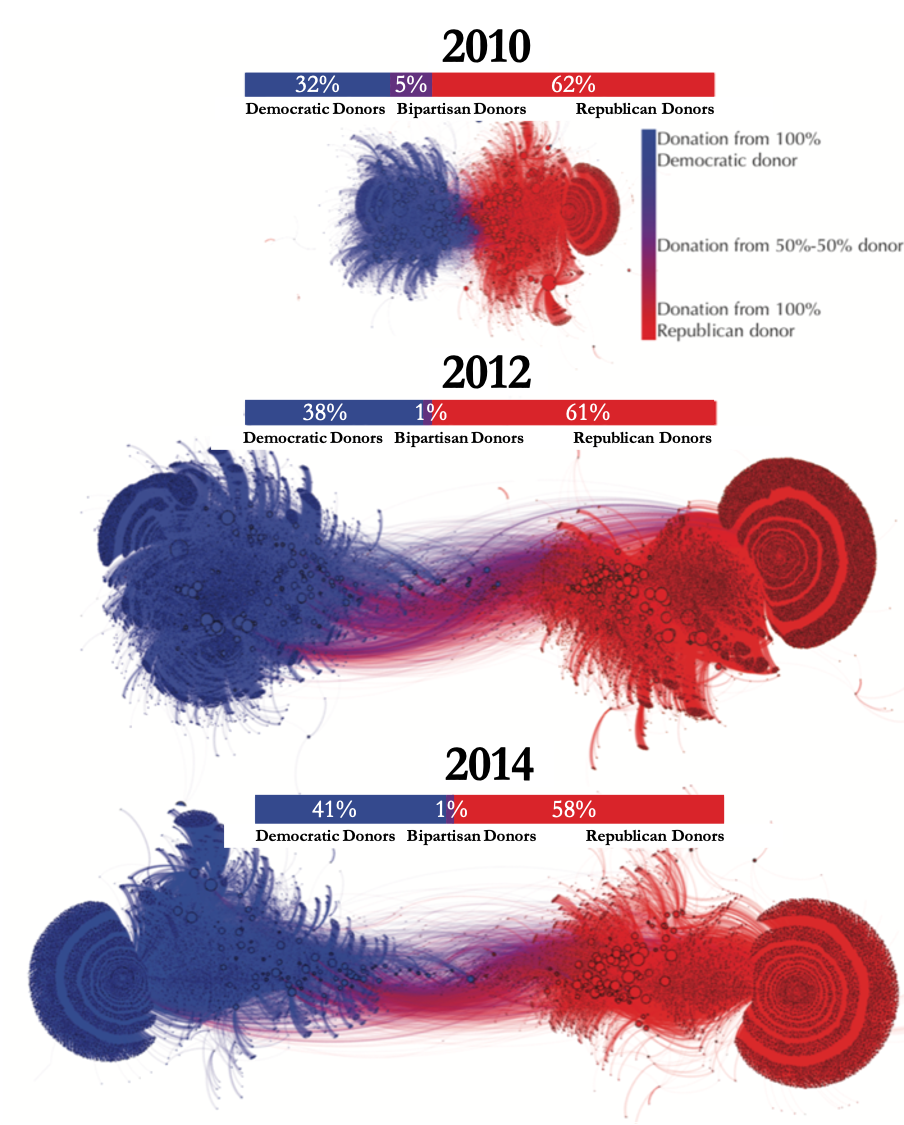
\includegraphics{../figures/fig1.png}
\caption{Fig. 1: Visual representation of Wisconsin donor networks in
the 2010, 2012 and 2014 election cycle using the Yifan Hu layout
algorithm. Percentages on the bars reprsent the percent of donors in
each party bin.}
\end{figure}

\hypertarget{references}{%
\section*{References}\label{references}}
\addcontentsline{toc}{section}{References}

\hypertarget{refs}{}
\leavevmode\hypertarget{ref-akey2015}{}%
Akey, Pat. 2015. ``Valuing Changes in Political Networks: Evidence from
Campaign Contributions to Close Congressional Elections.'' \emph{The
Review of Financial Studies} 28 (11): 3188--3223.

\leavevmode\hypertarget{ref-ansolabehere2003}{}%
Ansolabehere, Stephen, John M. de Figueiredo, and James M. Snyder Jr.
2003. ``Why Is There so Little Money in U.s. Politics.'' \emph{Journal
of Economic Perspectives} 17 (1): 105--30.

\leavevmode\hypertarget{ref-barber2016b}{}%
Barber, Michael J., Daniel M. Butler, and Jessica Preece. 2016. ``Gender
Inequalities in Campaign Finance.'' \emph{Quarterly Journal of Political
Science} 1 (2): 219--48.

\leavevmode\hypertarget{ref-barber2016c}{}%
Barber, Michael J., Brandice Canes-Wrone, and Sharece Thrower. 2016.
``Ideologically Sophisticated Donors: Which Candidates Do Individual
Contributors Finance.'' \emph{American Journal of Political Science} 61
(2): 1057--72.

\leavevmode\hypertarget{ref-blake2012}{}%
Blake, Aaron. 2012. ``Scott Walker Said Budget Strategy in Wisconsin Was
'Divide and Conquer'.'' \emph{The Washington Post}, May.

\leavevmode\hypertarget{ref-bode2018}{}%
Bode, Leticia, Stephanie Edgerly, Chris Wells, Itay Gabay, Charles
Franklin, Lew Friedland, and Dhavan V. Shah. 2018. ``Participation in
Contentious Politics: Rethinking the Roles of News, Social Media, and
Conversation Amid Divisiveness.'' \emph{Journal of Information
Technology \& Politics} 15 (3): 215--29.

\leavevmode\hypertarget{ref-bonica2017}{}%
Bonica, Adam. 2017. ``Professional Networks, Early Fundraising, and
Electoral Success.'' \emph{Election Law Journal: Rules, Politics, and
Policy} 16 (1): 153--71.

\leavevmode\hypertarget{ref-bonneau2007}{}%
Bonneau, Chris W. 2007. ``Campaign Fundraising in State Supreme Court
Elections.'' \emph{Social Science Quartlery} 88 (1): 68--85.

\leavevmode\hypertarget{ref-borsuk2017}{}%
Borsuk, Alan. 2017. ``New Poll Gives Vivid Look into Polarized Political
Perceptions.'' June 29, 2017.
\url{https://law.marquette.edu/poll/2017/06/29/new-poll-gives-vivid-look-into-polarized-political-perceptions/}.

\leavevmode\hypertarget{ref-bowler2015}{}%
Bowler, Shaun, and Todd Donovan. 2015. ``Campaign Money, Congress, and
Perceptions of Corruption.'' \emph{American Politics Research} 44 (2):
272--95.

\leavevmode\hypertarget{ref-bramlett2011}{}%
Bramlett, Brittany H., James G. Gimpel, and Frances E. Lee. 2011. ``The
Political Ecology of Opinion in Big-Donor Neighborhoods.''
\emph{Political Behavior} 33: 565--600.

\leavevmode\hypertarget{ref-pew2017}{}%
Center, Pew Research. 2017. ``The Partisan Divide on Political Values
Grows Even Wider.'' online.

\leavevmode\hypertarget{ref-conover2011}{}%
Conover, Michael D., Jacob Ratkiewicz, M. Francisco, B. Gonçalves, F.
Menczer, and A. Flammini. 2011. ``Political Polarization on Twitter.''
In \emph{ICWSM}.

\leavevmode\hypertarget{ref-cooper2010}{}%
Cooper, Michael J., Huseyin Gulen, and Alexei V. Ovtchinnikov. 2010.
``Corporate Political Contributions and Stock Returns.'' \emph{The
Journal of Finance} 65 (2): 687--724.

\leavevmode\hypertarget{ref-cramer2016}{}%
Cramer, K. J. 2016. \emph{The Politics of Resentment: Rural
Consciousness in Wisconsin and the Rise of Scott Walker}. Chicago
Studies in American Politics. University of Chicago Press.
\url{https://books.google.com/books?id=Rg2ZCwAAQBAJ}.

\leavevmode\hypertarget{ref-crowder-meyer2018}{}%
Crowder-Meyer, Melody, and Rosalyn Cooperman. 2018. ``Can't Buy Them
Love: How Party Culture Among Donors Contributes to the Party Gap in
Women's Representation.'' \emph{The Journal of Politics} 80 (4):
1211--24.

\leavevmode\hypertarget{ref-igraph}{}%
Csardi, Gabor, and Tamas Nepusz. 2006. ``The Igraph Software Package for
Complex Network Research.'' \emph{InterJournal} Complex Systems: 1695.
\url{http://igraph.org}.

\leavevmode\hypertarget{ref-ellis2017}{}%
Ellis, William Curtis, Joseph T. Ripberger, and Colin Swearingen. 2017.
``Public Attention and Head-to-Head Campaign Fundraising: An Examination
of U.s. Senate Elections.'' \emph{American Review of Politics} 36 (1):
30--53.

\leavevmode\hypertarget{ref-garro2020}{}%
Fowler, Anthony, Haritz Garro, and Jörg L. Spenkuch. 2020. ``Quid Pro
Quo? Corporate Returns to Campaign Contributions.'' \emph{The Journal of
Politics} 82 (3): 844--58.

\leavevmode\hypertarget{ref-francia2003}{}%
Francia, Peter L., John C. Green, Paul S. Herrnson, Lynda W. Powell, and
and Clyde Wilcox. 2003. \emph{The Financiers of Congressional
Elections}. New York, NY: Columbia University Press.

\leavevmode\hypertarget{ref-francia2005}{}%
Francia, Peter L., John C. Green, Paul S. Herrnson, Lynda W. Powell, and
Clyde Wilcox. 2005. ``Limousine Liberals and Corporate Conservatives:
The Financial Constituencies of the Democratic and Republican Parties.''
\emph{Social Science Quarterly} 86 (4): 761--78.

\leavevmode\hypertarget{ref-garcia2015}{}%
Garcia, David, Adiya Abisheva, Simon Schweighofer, Uwe Serdült, and
Frank Schweitzer. 2015. ``Ideological and Temporal Components of Network
Polarization in Online Political Participatory Media.'' \emph{Policy \&
Internet} 7 (1): 46--79.

\leavevmode\hypertarget{ref-gordon2007}{}%
Gordon, Sanford C., Catherine Hafer, and Dimitri Landa. 2007.
``Consumption or Investment? On Motivations for Political Giving.''
\emph{The Journal of Politics} 69 (4).

\leavevmode\hypertarget{ref-guerra2013}{}%
Guerra, P. H. Calais, Wagner Meira Jr., Clair Cardie, and R. Kleinberg.
2013. ``Party Polarization in Congress: A Network Science Approach.''
\emph{Proceedings of the 7th International Conference on Weblogs and
Social Media, ICWSM 2013}, January, 215--24.

\leavevmode\hypertarget{ref-harden2016}{}%
Harden, Jeffrey J., and Justin H. Kirkland. 2016. ``Do Campaign Donors
Influence Polarization? Evidence from Public Financing in the American
States.'' \emph{Legislative Studies Quarterly} 41 (1): 119--1542.

\leavevmode\hypertarget{ref-hill2017}{}%
Hill, Seth J., and Gregory A. Huber. 2017. ``Representativeness and
Motivations of the Contemporary Donorate: Results from Merged Survey and
Administrative Records.'' \emph{Political Behavior} 39 (March): 3--29.

\leavevmode\hypertarget{ref-kaufman2012}{}%
Kaufman, Dan. 2012. ``How Did Wisconsin Become the Most Politically
Divisive Place in America?'' \emph{The New York Times Magazine}, May.

\leavevmode\hypertarget{ref-keena2019}{}%
Keena, Alex, and Misty Knight-Finley. 2019. ``Are Small Donors
Polarizing? A Longitudinal Study of the Senate.'' \emph{Election Law
Journal: Rules, Politics, and Policy} 18 (2): 132--44.

\leavevmode\hypertarget{ref-kitchens2016}{}%
Kitchens, Karin E., and Michele L. Swers. 2016. ``Why Aren't There More
Republican Women in Congress? Gender, Partisanship, and Fundraising
Support in the 2010 and 2012 Elections.'' \emph{Politics \& Gender} 12
(4): 648--76.

\leavevmode\hypertarget{ref-laurison2016}{}%
Laurison, Daniel. 2016. ``Social Class and Political Engagement in the
United States.'' \emph{Sociology Compass} 10 (9): 684--97.

\leavevmode\hypertarget{ref-layton2011}{}%
Layton, Lyndsey. 2011. ``'Wisconsin 14' Group of Democratic Senators
Returns, Greeted by Thousands at Capitol.'' \emph{The Washington Post},
March.

\leavevmode\hypertarget{ref-marley2019}{}%
Marley, Patrick, and Molly Beck. 2019. ``Divisive Politics Ruled
Wisconsin over the Last Decade.'' \emph{Milwaukee Journal Sentinel},
December.

\leavevmode\hypertarget{ref-mccarty2006}{}%
McCarty, Nolan, Keith T. Poole, and Howard Rosenthal. 2006.
\emph{Polarizaed America: The Dancedance of Ideology and Unequal
Riches}. Cambridge, Mass: MIT Press.

\leavevmode\hypertarget{ref-newman2006}{}%
Newman, M. E. J. 2006. ``Modularity and Community Structure in
Networks.'' \emph{Proceedings of the National Academy of Sciences} 103
(23): 8577--82. \url{https://doi.org/10.1073/pnas.0601602103}.

\leavevmode\hypertarget{ref-palmer2008}{}%
Palmer, Vernon Valentine, and John Levendis. 2008. ``The Louisiana
Supreme Court in Question: An Empirical and Statistical Study of the
Effects of Money on the Judicial Function.'' \emph{Tulane Law Review} 82
(4): 1291--1314.

\leavevmode\hypertarget{ref-laraja2011}{}%
Raja, Raymond J. La, and David L. Wiltse. 2012. ``Don't Blame Donors for
Ideological Polarization of Political Parties: Ideological Change and
Stability Among Political Contributors, 1972-2008.'' \emph{American
Politics Research} 40 (3): 501--30.

\leavevmode\hypertarget{ref-roscoe2005}{}%
Roscoe, Douglas D., and Shannon Jenkins. 2005. ``A Meta-Analysis of
Campaign Contributions' Impact on Roll Call Voting.'' \emph{Social
Science Quartlery} 86 (1): 52--68.

\leavevmode\hypertarget{ref-sewell2011}{}%
Sewell, Abby. 2011. ``Protesters Out in Force Nationwide to Oppose
Wisconsin's Anti-Union Bill.'' \emph{Los Angeles Times}, February.

\leavevmode\hypertarget{ref-shor2015}{}%
Shor, Boris. 2015. ``Polarization in American State Legislatures.'' In
\emph{American Gridlock: The Sources, Character, and Impact of Political
Polarization}, edited by James A. Thurber and AntoineEditors Yoshinaka,
203--21. Cambridge University Press.
\url{https://doi.org/10.1017/CBO9781316287002.011}.

\leavevmode\hypertarget{ref-stratmann1991}{}%
Stratmann, Thomas. 1991. ``What Do Campaign Contributions Buy?
Deciphering Causal Effects of Money and Votes.'' \emph{Southern Economic
Journal} 57 (3): 606--20.

\leavevmode\hypertarget{ref-thomsen2017}{}%
Thomsen, Danielle M., and Michele L. Swers. 2017. ``Which Women Can Run?
Gender, Partisanship, and Candidate Donor Networks.'' \emph{Political
Research Quarterly} 70 (2): 449--63.

\leavevmode\hypertarget{ref-torres-spelliscy2017}{}%
Torres-Spelliscy, Ciara. 2017. ``Time Suck: How the Fundraising
Treadmill Diminishes Effetive Governance.'' \emph{Seton Hall Legislative
Journal} 42 (December).

\leavevmode\hypertarget{ref-waugh2009}{}%
Waugh, Andrew Scott, Liuyi Pei, James H. Fowler, Peter J. Mucha, and
Mason Alexander Porter. n.d. ``Party Polarization in Congress: A Network
Science Approach.''

\leavevmode\hypertarget{ref-zhang2008}{}%
Zhang, Yan, A. J. Friend, Amanda L. Traud, Mason A. Porter, James H.
Fowler, and Peter J. Mucha. 2008. ``Community Sructure in Congressional
Cosponsorship Networks.'' \emph{Physica A: Statistical MEchanics and Its
Applications} 387 (1): 1705--12.





\newpage
\singlespacing 
\end{document}
